%!TEX TS-program = xelatex
\documentclass[12pt]{article}
\usepackage[english]{babel}
\usepackage[square,sort,comma,numbers]{natbib}
\usepackage{url}
\usepackage{amsmath}
\usepackage{graphicx}
\usepackage{float}
\usepackage[font=footnotesize]{caption}
\usepackage{vmargin}
\usepackage[super]{nth}

%Unidades SI
\usepackage[seperr]{siunitx}
\usepackage{mathtools}
\usepackage{setspace}
\usepackage{fontspec}
\usepackage{xcolor}
\usepackage{titlesec}
\usepackage{parskip}
\usepackage{subfig}
\usepackage{fancyhdr}
\usepackage[nodayofweek]{datetime}
\usepackage{afterpage}

\usepackage{lipsum}

\setsansfont[Ligatures=TeX]{ArialB.ttf}

\fancypagestyle{plain}{
  \renewcommand{\headrulewidth}{0pt}
  \fancyhf{}
  \fancyfoot[C]{\footnotesize Page \thepage}
}

%definir o estilo dos titulos das secções
\titleformat*{\section}{\vspace{12pt}\fontsize{14}{6}\sffamily}
\titleformat*{\subsection}{\vspace{12pt}\fontsize{14}{6}\sffamily}


\onehalfspacing


%definir as margens
\setmarginsrb{2 cm}{1 cm}{2 cm}{2 cm}{0.5 cm}{0.5 cm}{1.5 cm}{1 cm}

\captionsetup[figure]{labelsep=endash}
\captionsetup[table]{labelsep=endash}

\setcounter{section}{0}

\fancypagestyle{title1}
{
    \renewcommand{\headrulewidth}{0pt}
    \fancyhf{}
    \fancyfoot[C]{\today}
}

\usepackage{anyfontsize}

\addto\captionsportuguese{
\renewcommand{\figurename}{Fig.}
}

\addto\captionsportuguese{
\renewcommand{\tablename}{Tab.}
}

%\DeclareMathAlphabet{\mathtt}{OT1}{pbk}{m}{n}

\setmathtt{Arial.ttf}

\begin{document}

    \setmainfont[Ligatures=TeX]{ArialB.ttf}

    \begin{titlepage}
        \thispagestyle{title1}
        \flushleft
        
\includegraphics[scale = 0.3]{imagens/ist.png}\\[1.5 cm]
        \centering
        \textsc{\fontsize{18}{22}\selectfont INSTITUTO SUPERIOR TÉCNICO}\\[2 cm]
        \textsc{\fontsize{22}{25}\selectfont BIG DATA MEASURING SYSTEMS}\\[3 cm]
        \textsc{\fontsize{22}{25}\selectfont VIBRATION ANALYSIS EXPERIMENT:}\\[0.1 cm]
        \mbox{\textsc{\fontsize{22}{25}\selectfont FORM SIGNALS TO CLOUD SENSOR PLATFORM }}\\[3 cm]
        \textsc{\fontsize{28}{34}\selectfont Formal Report}\\[5 cm]
        \begin{minipage}{0.5\textwidth}
            \quad
        \end{minipage}
        \setmainfont[Ligatures=TeX]{Arial.ttf}
        \begin{minipage}{0.49\textwidth}
            ist194942 -- Paolo Frazzetto\\[2cm]
            Prof. Luís Rosado
        \end{minipage}
\end{titlepage}

\setmainfont[Ligatures=TeX]{Times.ttf}

\newpage

\pagestyle{plain}

\section{Introduction}
This report describes the \nth{3} and \nth{4} laboratory experiences carried out for the course \emph{Big Data Measuring Systems} during April and May 2020 at IST, Lisbon \cite{1}. This experiment simply demonstrates how to deal with all the relevant aspects concerning the field of Big Data: signal acquisition and digitalization; data storage and analysis; cloud upload and visualisation.

Sensors transform a specific physical quantity into a electric signal. This information is then translated into the digital domain, characterised by discrete time and binary-represented amplitudes, in order to exploit the advantages of digital systems and transmissions. Dedicated algorithms further process this information to get the features of interest, suited to be stored for a later use. Cloud computing can be used to deal with different distributed and remote sensors by providing monitoring dashboards, computing post-processing data analytics and eventually allowing to plan for future control and maintenance of the devices.

The studied problem consists of analysing the vibrations of a wheel placed on a motor axis to infer its state and conditions. The analogue signal is captured by means of an accelerometer, that is later digitalized using a microcontroller. The signal is then read and pre-processed by specific algorithms that extract the desired quantities, before they are uploaded to a cloud sensor platform for the final analysis and visualisation. 

\section{Equipment}	
Due to external and unforeseen circumstances, it was not possible to directly access the laboratory and its equipment. Therefore, all the presented results are based on a virtual signal generator provided by the faculty, that mimics the actual signal acquisition and digitalization for different tunable settings. Another virtual black-box signal generator was provided to simulate unknown working conditions.
\begin{itemize}
	\item Tunable virtual signal generator that simulates \cite{setup}:
		\begin{itemize}
			\item signal generator Leader LFG 1320;
			\item 12 V 37Dx54L 50:1 motor with a 90 mm wheel;
			\item ADXL337 accelerometer;
			\item connection board NICB68-LP;
			\item DAQ National Instrument NI6220;
		\end{itemize}
	\item Virtual black-box signal generator;
	\item PC with Matlab software and Data Signal Processing toolbox \cite{DSP};
	\item ThingSpeak channels and online Matlab App \cite{TS}.
\end{itemize}

\section{Apparatus Behaviour}
A primary investigation of the setup inner workings is done by setting the power supply at 12 V (with 0 g unbalancing weight and 100 \% health conditions) and by acquiring the accelerometer signal of the X axis. To capture all the information and to guarantee a proper digital signal reconstruction respecting the Nyquist-Shannon sampling theorem, at each acquisition the input range is set at $\pm$ 2 V, the sampling rate at $f_s=1$ kHz and 10 000 points are being sampled. This finite sequence of sample is converted to its frequency domain representation by means of the Discrete Fourier Transform (DFT). This first output is shown in Fig.~\ref{fig:refsignal}.	    
	\begin{figure}[h]
	   	\centering
	   	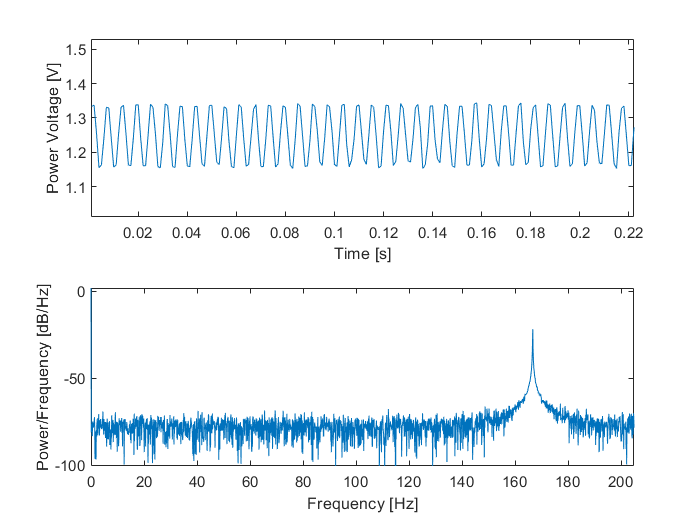
\includegraphics[width=0.9\linewidth]{Figures/RefSignal}
	   	\caption{Detail of the acquired signal and its spectrum at standard working conditions: 12 V power supply, 0 g weight and 100 \% health.}
	   	\label{fig:refsignal}
	\end{figure}
In the time domain, the signal RMS is at 1.251 V while the RMS of the AC component, that is equivalent to the signal standard deviation, directly comes from the motor vibrations and is equal to 0.071 V. The two RMS are related by
\begin{equation}
RMS_{AC+DC}=\sqrt{RMS^2_{DC}+RMS^2_{AC}}.
\end{equation} 
Having a look at the spectrum, the maximum frequency is peaked at 166.7 Hz. Thus, the signal is composed of frequencies below the maximum permitted frequency by the Nyquist-Shannon theorem, namely $f_s/2=500$ MHz. Notice also that spectral leakage arises from sampling not an integer multiple of signal periods. 

Different behaviours of the apparatus can be inspected by tuning the parameters of the provided signal generator within a certain range, namely the power supply from 1 V to 15 V, the unbalancing weight from 0 g to 100 g and the motor state of health from 0 \% to 100 \%. By fixing two of them and varying the third one it is possible to design algorithms able to estimate the motor status from the acquired spectra. 
	\subsection{Rotation Speed Estimation}
	The feature related to the rotation speed is the frequency of the peak at the highest frequencies. As shown in Fig.~\ref{fig:voltagefeature}, its value follows a linear relation dependent on the supplied power according 
	 	\begin{equation}
	 		f_{MaxPeak} = 13.9\cdot Voltage-6\times 10^{-3}.
	 	\end{equation}
   	This frequency corresponds to the rotation of the motor main axis that has a 50:1 gear ratio. This means that once $f_{MaxPeak}$ is extracted from the signal spectrum, the wheel rotates at $f_{MaxPeak} / 50$ Hz or $(f_{MaxPeak}\times 60)/50$ rpm.
   		\begin{figure}[h]
	   		\centering
	   		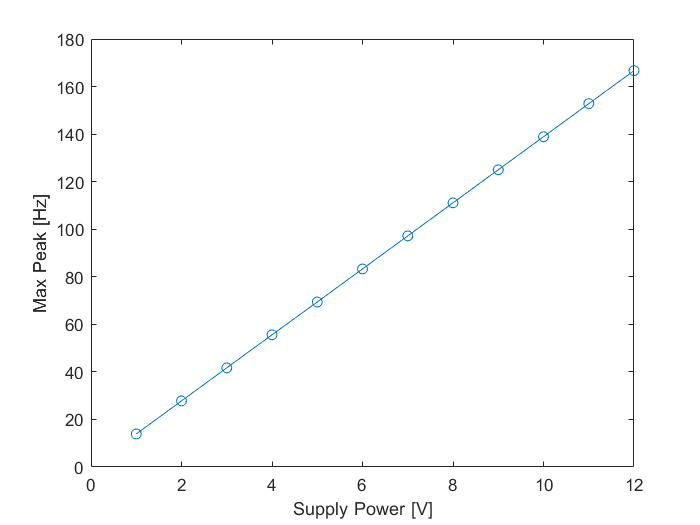
\includegraphics[width=0.9\linewidth]{Figures/VoltageFeature}
	   		\caption{Linear interpolation for different power supply voltages in [1,12] and corresponding frequency of the peak at higher frequency.}
	   		\label{fig:voltagefeature}
   		\end{figure}
	\subsection{Unbalancing Weight Estimation}
	It is possible to fix a load on the wheel with a screw, causing the axis unbalance. By fixing the input supply at 12 V an varying the weight, another peak at $\approx\ $3 Hz emerges, that is indeed the expected rotation frequency of the wheel for that supplied power. Fig.~\ref{fig:weightfeature} shows the relation between these two quantities that is purely linear: the heavier the weight, the higher the amplitude of the peak at low frequencies.
		\begin{figure}[h]
			\centering
			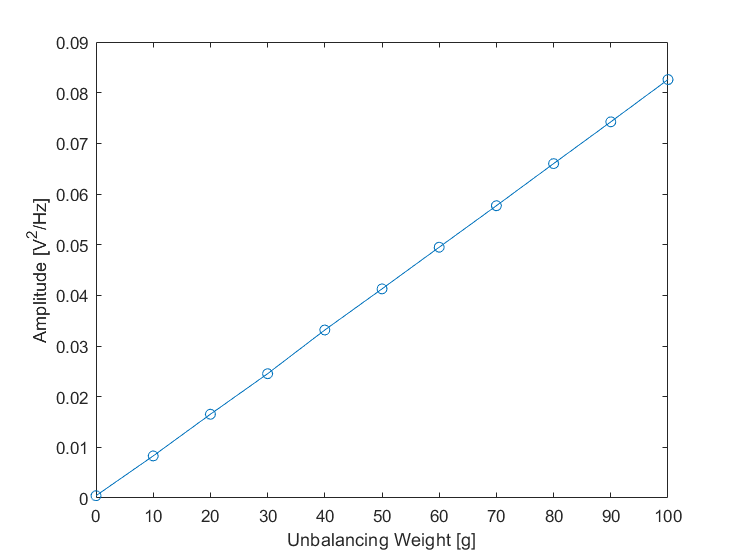
\includegraphics[width=0.9\linewidth]{Figures/WeightFeature}
			\caption{Linear interpolation for different weights and amplitude of the peak at low frequency. The power supply is set at 12 V.}
			\label{fig:weightfeature}
		\end{figure}
	The two quantities are related by
	\begin{equation}\label{eq:weight}
	Amplitude\bigr|_{f\approx 3 \text{Hz}} = 8.25 \times 10^{−4}\cdot Weight - 8.5\times 10^{−6}.
	\end{equation}
	To take into account what happens at different rotation speeds, remember the expression for the centrifugal force
	\begin{equation}
		F_c = mr\omega^2	
	\end{equation}
	and its quadratic dependence on the angular velocity $\omega$. This is modelled as	
	\begin{equation}\label{eq:feature2}
		Amplitude\bigr|_{f\approx 3 \text{Hz}} = \left(k_1\cdot Weight\right)\left(k_2\cdot Speed\right)^2
	\end{equation}
	where $k_1 = 8.25 \times 10^{−4}\ [V^2/\left( Hz \cdot g\right)]$ is the slope of Eq.~\eqref{eq:weight} and $k_2 = 0.31\ [Hz^{-1}]$ can be estimated, for instance, by looking at the evolution of the amplitude at a fixed $Weight = 100$ g and changing the speed, as reported in Fig.~\ref{fig:weightfeaturespeed}. So by knowing the rotation speed and amplitude of the peak at low frequencies, it is possible to evaluate the weight of the load screwed on the wheel by inverting Eq.~\eqref{eq:feature2}.
	\begin{figure}[h]
		\centering
		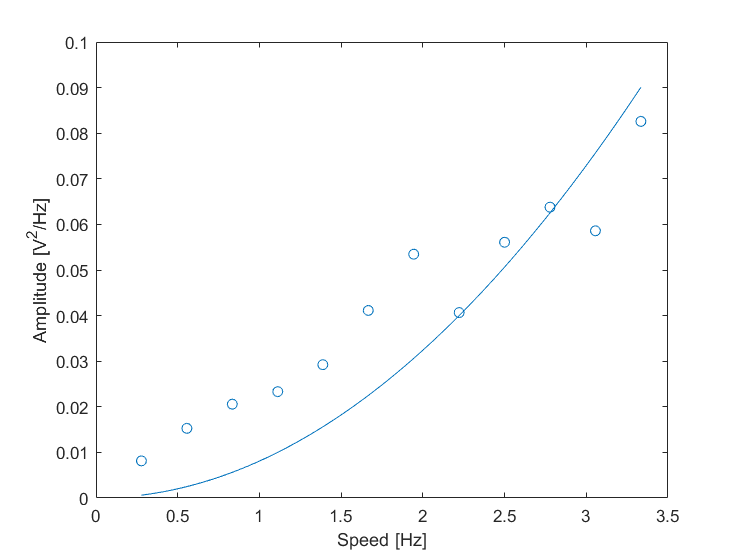
\includegraphics[width=0.9\linewidth]{Figures/WeightFeatureSpeed}
		\caption{Relation between the amplitude of the peak at the lowest frequencies and rotation speed with a fixed 100 g unbalancing weight. The fitted curve follows the centrifugal force formula.}
		\label{fig:weightfeaturespeed}
	\end{figure}
	\subsection{Motor Health Condition Estimation}
	Any motor undergoes the effects of ageing and worsening of the performances. In this case, the vibrations for a simulated worst case scenario (12 V, 100 g weight load and 0 \% health) are presented in Fig.~\ref{fig:worstcase}. 
	\begin{figure}[h]
		\centering
		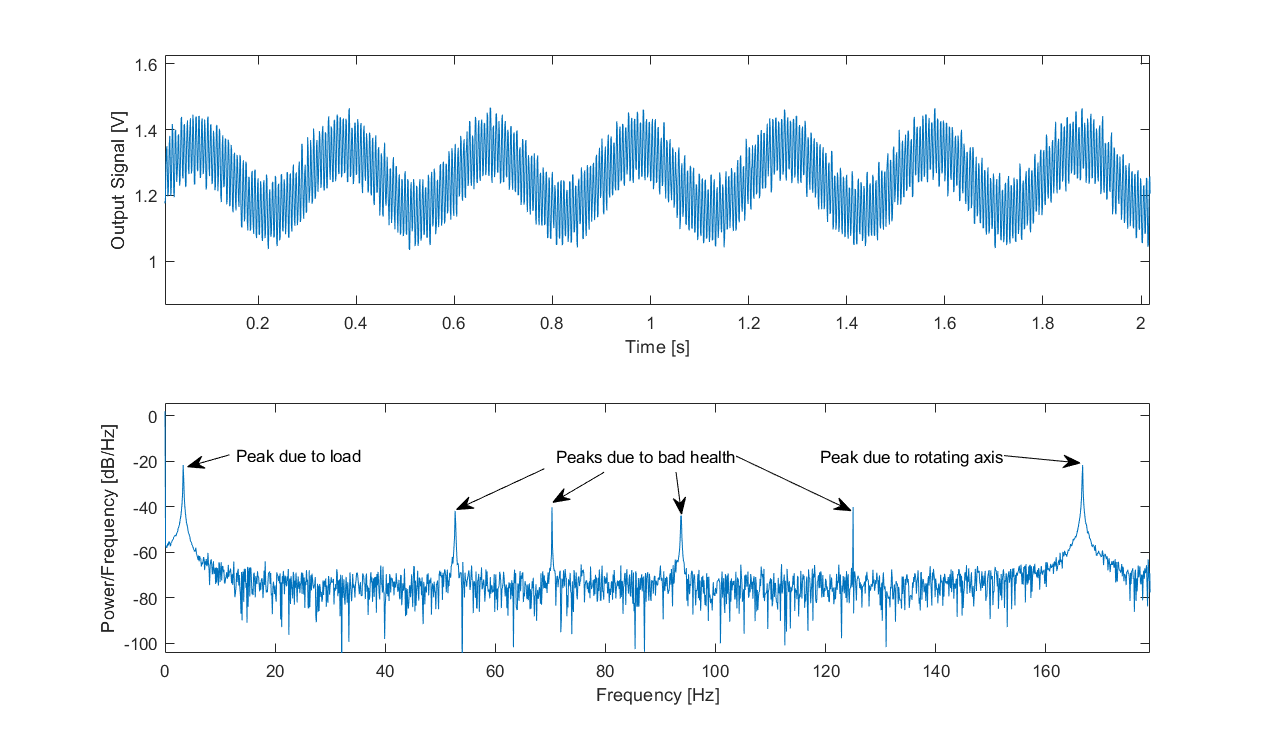
\includegraphics[width=0.9\linewidth]{Figures/WorstCase}
		\caption{Aquired signal and its spectrum at worst simulated conditions: 12 V power supply, 100 g weight load and 0 \% health.}
		\label{fig:worstcase}
	\end{figure}
	Besides the peaks corresponding to the rotating axis and spinning load already discussed, bad health conditions give rise to 4 additional vibration modes below the rotating axis frequency. The ratio among them and the rotating axis frequency is in fact 0.75, while their amplitude is proportional to the health status as shown in Fig.~\ref{fig:healthfeature}. 
	\begin{figure}[h!]
		\centering
		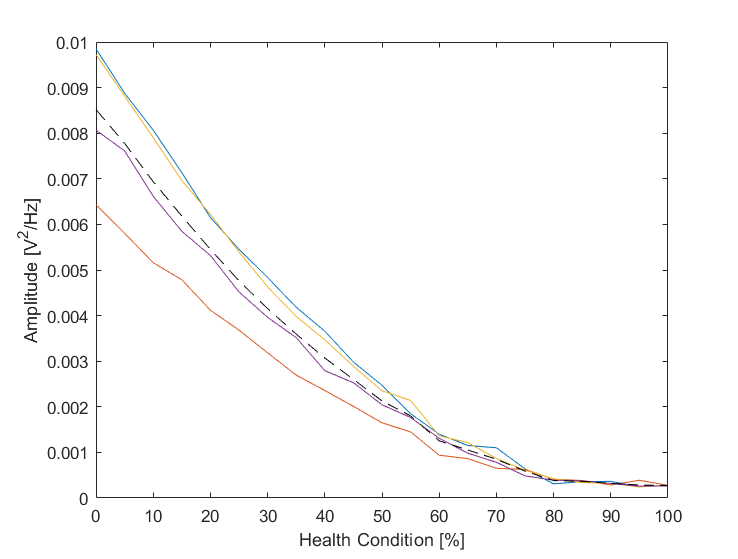
\includegraphics[width=0.9\linewidth]{Figures/HealthFeature}
		\caption{Amplitude and average (dashed line) of the 4 peaks related to the health condition. At a fixed health, the order of the peaks amplitude follows the order of their corresponding frequencies (i.e. the lowest line corresponds to the amplitude of the peak at lowest frequency and so on.)}
		\label{fig:healthfeature}
	\end{figure}
	This feature allows to discern the health status only when it is $\leq\ $ 70 \% since above that these peaks are hidden by noise. Moreover, for a fixed health the amplitude increases with the frequency, therefore their average is considered as reference feature and it is used for a linear interpolation, yielding to
	\begin{equation}
	\overline{Amplitude}\bigr|_{\text{Health}\leq 70 \%} = -1.11\times10^{-4}\cdot Health + 7.89\times 10^{-3}.
	\end{equation}
	This first model does not take into account the effect of different rotation speeds and the consequent shift of the maximum rotating axis frequency. Similarly to the weight estimation procedure, the average amplitude rather follows the quadratic expression
	\begin{equation}\label{eq:feature3}
	\overline{Amplitude}\bigr|_{\text{Health}\leq 70 \%} = \left( k_3\cdot\left( Health - 100\right) \right)^2\left( k_4\cdot Speed\right) 
	\end{equation}
	where $k_3= 2.06\times10^{-2}$ and $k_4 = 6.11\times 10^{-4}\ [V^2/Hz^2]$.\\
	$k_4$ is obtained as the slope of the average amplitude when changing speed at arbitrarily-chosen 50 \% health conditions. Once this coefficient is known, $k_3$ can be estimated by looking at the evolution of the average amplitude when changing the health, at an arbitrary fixed power supply of 12 V (i.e. the wheel is rotating at 3.3 Hz).
	
	The procedures described in this section followed by the inversion of Eq.~\eqref{eq:feature3} provide thus a guess of the health conditions of the motor only from the analysis of its vibration spectrum.
\section{Cloud Integration}
One approach to deal with distributed equipment and remote control is by using cloud sensing platform. ThingSpeak \cite{TS} is a popular and free service that provides all the necessary backend and frontend resources. Additionally, it is well integrated with Matlab thanks to a dedicated API and it allows for online execution of scripts.

Another signal generator supplied by the faculty simulates a real case scenario where the motor follows a unknown working cycle. Once the significant features are extracted from its spectrum, the cloud platform can then be employed to evaluate and display the quantities of interest to eventually trigger necessary maintenance actions. 
\subsection{Features Upload}
The first preprocessing of the signal consists of retrieving its spectrum by means of the DFT. Next, it is necessary to look for the required features. Recall that
\begin{itemize}
	\item Feature 1 is the maximum frequency, that is related to the rotation speed. It can be easily obtained from the spectrum peaks;
	\item Feature 2 is the amplitude of the peak at $\approx$ 3 Hz, form which the weight can be extracted. Since such a peak would not be present if there is no screwed weight, if the maximum amplitude in the range $[1,5]$ Hz is $\leq$ 0.05 (an arbitrary threshold) this feature is set to zero;
	\item Feature 3 is the average of the amplitude of the 4 peaks present in between feature 1 and the frequency of feature 2. If the average of the four highest amplitude in this range is $\leq$ 0.001 (i.e. is not statistically significant w.r.t noise) then the health cannot be estimated, meaning that it must be $\geq$ 70 \% and it is then naively gauged at 100 \%.
\end{itemize} 	
A Matlab scrip reads the signal from the black-box generator and extracts these features every 30 s. At each iteration, they are uploaded to a specific ThingSpeak channel (ID~1058393) thanks to the REST API. The feature channel final view is shown in Fig.~\ref{fig:TSFeatures}.
\begin{figure}[h!]
	\centering
	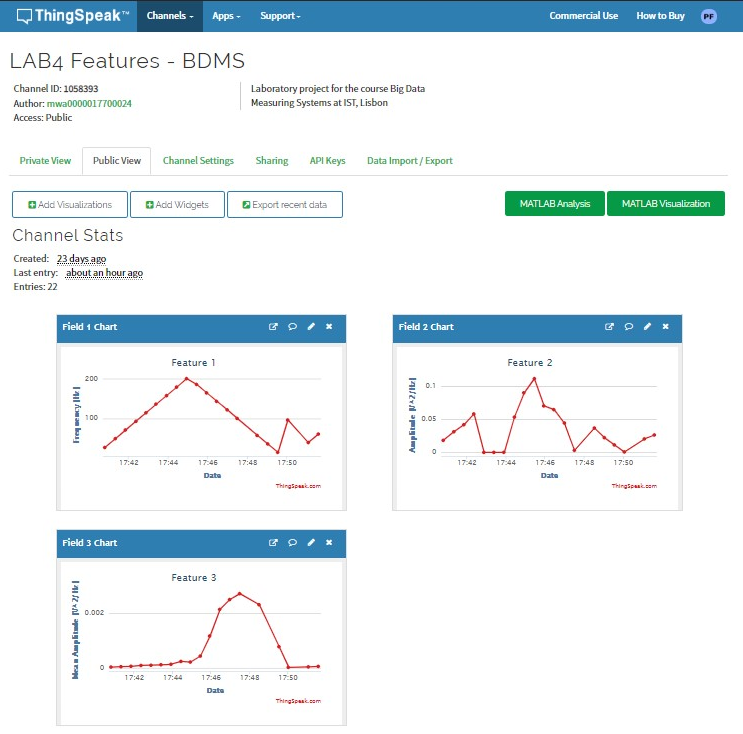
\includegraphics[width=0.9\linewidth]{Figures/TSFeatures}
	\caption{Screenshot of the features channel.}
	\label{fig:TSFeatures}
\end{figure}
\subsection{Final Analysis and Visualisation}
An online Matlab App takes care of the last post-processing. It gets the features from the features channel, it applies the algorithms described in Section~3 to get the motor state variables (wheel rotation speed, unbalancing weight, health conditions) and finally it uploads them to another channel (ID~1065024) that acts as a ``Customer View'', displayed in Fig.~\ref{fig:TFCustomer}.
\begin{figure}[t!]
	\centering
	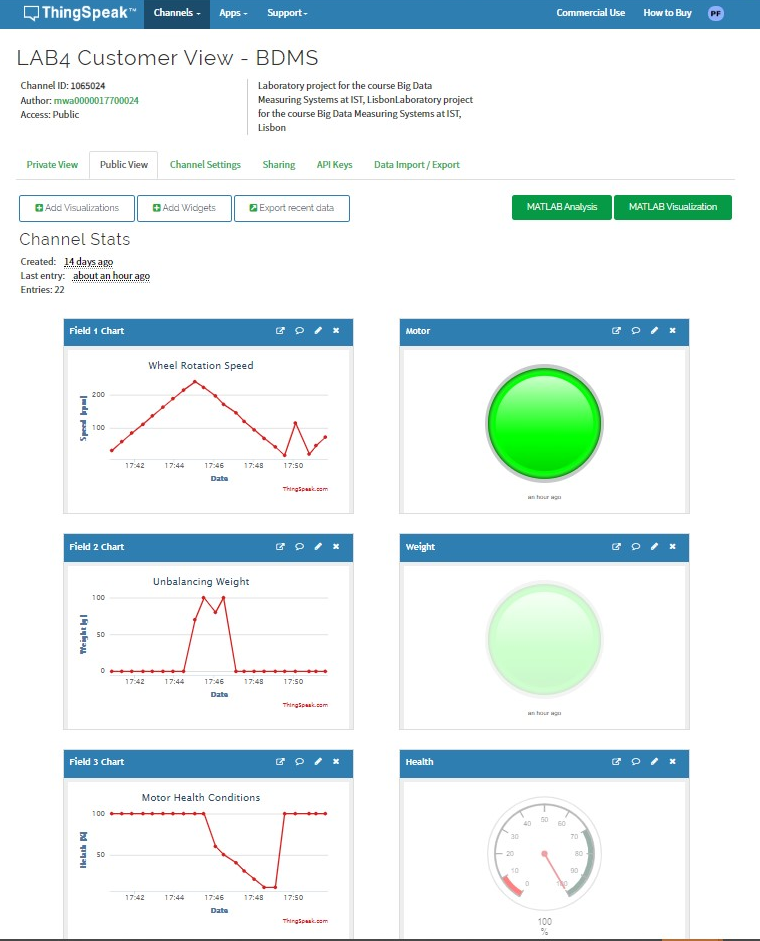
\includegraphics[width=0.9\linewidth]{Figures/TFCusomer}
	\caption{Screenshot of the custumer view channel. Along the variable charts, it contains lamp indicator or gauge for each motor state variable for monitoring purposes.}
	\label{fig:TFCustomer}
\end{figure}
This last channel has monitoring dashboards containing charts for each variables and lamp indicators to tell if the motor is powered (Speed $\geq$ 20 rpm) or if the weight is $\geq$ 50~g. It has also a gauge widget for the health condition.
Fig.~\ref{fig:TFCustomer} suggests as well that the cycle is $\approx$ 10 minutes long before it repeats itself. The rotation speed increases linearly until half cycle, then it decreases with the opposite slope until it stops. Before starting the new cycle though, there is a sudden and brief activation of the motor, found also in the Feature~1 chart of Fig.~\ref{fig:TSFeatures}. It is not clear whether this is an error of the feature extractions or it is made on purpose, a deeper investigation on the original spectrum would be required. Although Feature~2 is irregular, the estimation of the weight, corrected with the speed, shows that the load is added while the wheel is spinning at its fastest. The estimated weight is firstly 80 g and after one minute it
reaches 100 g. However, the post-processed points are noisier and also considering the poor quality of the fit of Fig.~\ref{fig:weightfeaturespeed}, a better model would be needed to get a more accurate estimate. Concerning the health, it is at top
conditions on the first half of the cycle and then it decreases exponentially to 10 \%.
\afterpage{\clearpage}  
\section{Conclusion}
The experiment has been carried out successfully. This report illustrates how to analyse and discuss spectra from different signals, while dealing with spectral leakage and Nyquist Theorem too. It is also presented how to characterize a physical experiment and design algorithms to guess its relevant features from the raw acquired data. The feature extraction is well
integrated in the ThingSpeak platform by means of a dedicated API. Moreover, cloud computing is used to post-process the features and display them in a online dashboard, similarly to what happens in real life scenarios.
\clearpage
\begin{thebibliography}{9}
\bibitem{1}
Big Data Measuring Systems, \url{https://fenix.tecnico.ulisboa.pt/disciplinas/SMGE/2019-2020/2-semestre/pagina-inicial}, Luís Rosado, 2020 IST
\bibitem{setup}
For all the documentation and detailed setup (not actually used), consult the Big Data Measuring System Webpage, 2020 IST
\bibitem{DSP}
MathWorks, Matlab Digital Signal Processing toolbox,  \url{https://www.mathworks.com/solutions/dsp.html}
\bibitem{TS}
ThingSpeak IoT analytics platform, \url{https://thingspeak.com/}
\end{thebibliography}

\end{document}